% file: 3-7-sssp/dijkstra-negative-edge.tex

\documentclass[tikz]{standalone}
\usetikzlibrary{shapes, positioning, fit}

\begin{document}
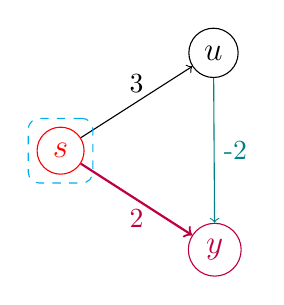
\begin{tikzpicture}[vertex/.style = {draw, circle, minimum size = 8pt, font = \large},
  node distance = 0.8cm and 1.5cm,
  every edge/.style = {draw, ->}]
  \node (s) [vertex, red] {$s$};

  \node (u) [vertex, above right = of s] {$u$};
  \node (y) [vertex, below right = of s, purple] {$y$};

  \path (s) edge node [above] {$3$} (u)
	    edge[purple, thick] node [below] {$2$} (y)
	(u) edge[teal] node [right] {-2} (y);

  \node [draw, rectangle, rounded corners, fit = (s), inner sep = 3pt, cyan, dashed] {};
\end{tikzpicture}
\end{document}
